\documentclass[UTF8,a4paper,15pt,titlepage,scale=0.8]{article}

\usepackage[a4paper]{geometry} 
\usepackage{fancyhdr}
\usepackage{amsmath}
\usepackage{graphicx}
\usepackage{color}
\usepackage{enumerate}
\usepackage{amssymb}
\usepackage{siunitx}
\usepackage{indentfirst}
\usepackage{pgfplots}
\usepackage{graphicx} 
\usepackage{float} 
\usepackage{subfigure}
\usepackage{mathtools}
\usepackage{mhchem}
\usepackage{tensor}
\usepackage[colorlinks,linkcolor=blue]{hyperref}


\pgfplotsset{width=10cm,height=7cm,compat=1.13} 


\definecolor{grey}{rgb}{0.85,0.85,0.85}

\graphicspath{Pictures/}

\setlength{\parindent}{2em}

\begin{document}
\begin{center}
    \large{\textbf{The Probability Analysis Behind the Random Tick Update in Minecraft}}
\end{center}
\begin{center}
    \textit{By: Runaway\_Fancy}
\end{center}

\tableofcontents
\section{Write in Front}
    This article is mainly explain the mechanics of random tick under Minecraft java edition. This small really takes lots of my times as the final exam is in the next week. I would like to use English to describe for my favor. So, it's arduous for Chinese players to read it over. But, actually, I would appreciate if you could find helpful parts for you and your machines. 
\section{Chunk Tick}
    \subsection{Chunks, Sub-chunks}
        Before we start, we should know the structure of chunk and sub-chunk. A chunk contains $16\times 16 \times 256$ blocks starting from layer $y=0$ to $y=256$(before 1.17). A sub-chunk is constructed by $16\times 16\times 16$ blocks forms a cubic. Each chunk contain 16 sub-chunks.
    \subsection{Definition}
        Chunk tick is one type of the cycle of the game. It happens inside a cylinder with horizontal cross section parallel to the horizontal surface with radius $R = 128$ blocks and central chunk ticking as \textbf{entity ticking}. \textbf{The block inside the ticking chunks are ticked on every game tick}.
    \subsection{Example of Events Controlled by Chunk Tick update}
        There are some events will happen if chunks gets ticked\cite{ref1}.
            \begin{enumerate}[$\cdot$]
                \item Mob naturally spawn.
                \item During a thunderstorm, lightning may strike somewhere in the chunk.
                \item If in a cold biome, water freezes into ice if possible.
                \item If snowing, a snow layer is placed if possible(cauldrons can be filled with powder snow, in 1.17).
                \item A certain number of blocks within the chunk receive random block ticks, that is what we focus on.
            \end{enumerate}
\section{Random Tick}
    \subsection{Definition}
        Random tick can be considered as a special case of chunk tick. It happens in every sub-chunks that inside the ticked chunks. The mechanics of this random tick update is(under the rate equal to 3)
            \begin{center}
                \textit{Randomly select three blocks in one sub-chunks and give them random tick update}
            \end{center}
        Default value of random tick rate is 3. Players could also use command \textit{/gamerule randomTickSpeed <value>} to switch the random tick rate. There is one particular case that even though some blocks are out of the range of the ticking cylinder, it can also receive random tick update.
    \subsection{Random Tick Dependent Blocks}
        Most of blocks do not affect by random tick update. But some use it to do something\cite{ref1}. 
            \begin{enumerate}[$\cdot$]
                \item Crops may grow or uproot.
                \item Mushrooms may spread or uproot.
                \item Vines may spread.
                \item Fire may burn out or spread.
                \item Ice and snow layers may melt.
                \item Leaves may decay.
                \item Farmland hydration is updated.
                \item Cacti, sugar cane, kelp, bamboo, chorus flowers and sweet berry bush may grow.
                \item Grass blocks and mycelium may spread.
                \item Grass blocks, mycelium, and nylium may decay (if and only if the condition is met).
                \item Saplings may grow into a tree.
                \item Lava may set fires nearby.
                \item Lit redstone ore turns off.
                \item Turtle eggs crack or hatch.
                \item Campfire smoke appears.
            \end{enumerate}
\section{Random Tick Update inside One Sub-chunk}
    It seems that random tick is a total random thing that we are forceless to control this thing. But we could use statical analysis to predict the tendency of random tick or use probability and expectation value to make our decision.
    \subsection{The Probability Distribution Model of Random Tick Update}
        For a random block in one sub-chunk, the probability that one random observed block is ticked is 
            \begin{equation}
                p = \frac{3}{\Omega}
            \end{equation}
        Where $\Omega = 16^3$. Assuming the random variable $K$ represents "The number of a random block be ticked". For observing time period t, we have 
            \begin{equation}
                K \sim b(t,p)
            \end{equation}
        The probability mass function of $K$ is
            \begin{equation}
                P(K=k)(t) = C_k^{t}p^{k}(1-p)^{t-k}
            \end{equation}
        Where 
            \begin{equation}
                C_k^t = \frac{t !}{k !(t-k) !}
            \end{equation}
        The cumulative distribution function is
            \begin{equation}
                C(t) = \sum_j^{t}P(K=k)(j)
            \end{equation}
        Or using poisson distribution($\Omega$ is big enough, binomial distribution can approximate to poisson distribution).
    \subsection{Modification of our Model}
        We aware that there is period form the last ticking to the end of observation which equivalently is doing nothing. So, to maximize the efficient, we cloud change a little bit on our probability model
            \begin{equation}
                P(K=k)(t) = C^{t-1}_{k-1}p^k(1-p)^{t-k}
            \end{equation}
        This is known as \textbf{negative binomial distribution}. That means we fixed our $t^{th}$ observation whose result is "ticking". After achieving our quota, we stop observing. 
\section{In Real Application - Modify the Construction of Random Tick Depended Farm}
    \subsection{Condition probability}
        In real cases, some blocks inside one sub-chunks is not our targets, e.g. a cocoa farm may contain $n$ cocoa-beans in one sub-chunk($n\geq 3$). Assuming random variable $X$ represents the number of cocoa were ticked. $X \sim G(3,\Omega)$, the probability distribution is listed in table 1.
            \begin{table}[H]
                \centering
                \begin{tabular}{c|c|c|c|c}
                    \hline
                    Notation&$p_0$&$p_1$&$p_2$&$p_3$\\
                    \hline
                    $X$&0&1&2&3\\
                    \hline
                    $P(X=x)$&$\frac{C_3^{\Omega-n}}{C_3^{\Omega}}$&$\frac{C_2^{\Omega - n}C_1^n}{C_3^{\Omega}}$&$\frac{C_1^{\Omega-n}C_2^n}{C_3^{\Omega}}$&$\frac{C_3^n}{C_3^{\Omega}}$\\
                    \hline
                \end{tabular}
                \caption{G.D. for $n\ge 3$}
            \end{table}
        If we observe a random cocoa bean $a_i$, the conditional probability $P(a_i| X=b)$ means "The probability of ticking $a_i$ under the condition only tick $b$ cocoa beans totally". So we have 
            \begin{equation}
                P(\text{ticking $a_i$ and only tick b cocoa beans}) = \frac{b}{n}p_b \ \ (b=0,1,2,3)
            \end{equation}
        The total probability that a random cocoa bean is ticked 
            \begin{equation}
                P_\Sigma = 0.2 (\frac{1}{n}p_1 + \frac{2}{n}p_2 + \frac{3}{n}p_3)
            \end{equation}
        The factor $0.2$ is the probability tha the cocoa bean change its level when received one random tick.
    \subsection{General Formula}
        The general formula of calculate the productive efficiency is
            \begin{equation}
                \Gamma (t) = \frac{C(t)}{t} \times N\gamma\epsilon
            \end{equation}
        Where 
            \begin{equation}
                C(t) = \sum_{j=m}^t P(M=m,j)
            \end{equation}
            \begin{equation}
                P(M=m,j) = C_{m-1}^{j-1} p_{\Sigma}^m(1-p_\Sigma)^{j-m}
            \end{equation}
            \begin{equation}
                P_{\Sigma} = r(\frac{1}{n}p_1 + \frac{2}{n}p_2 + \frac{3}{n}p_3)
            \end{equation}
        For $P_i$, seen in table 1. $r$ here means the probability that the target block change level after receive one random tick. $m$ means the number of successfully update. $M$ is random variable. $N$ is the number of the block per sub-chunk. $\gamma$ is drop rate. $\epsilon$ is collected rate.

        Here we provide a MATLAB script to help players to calculate and find the critical point of $\Gamma(t)$, see figure 1.
            \begin{figure}[H]
                \centering
                \subfigure[MATLAB program to calculate the maximum of $\Gamma(t)$]{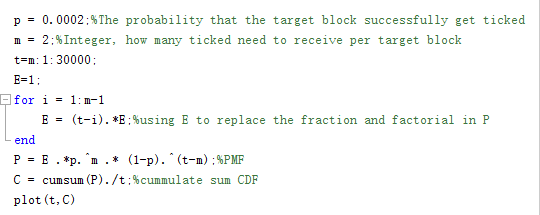
\includegraphics[width=0.45\textwidth]{MLAB program.png}}
                \subfigure[Result of this example]{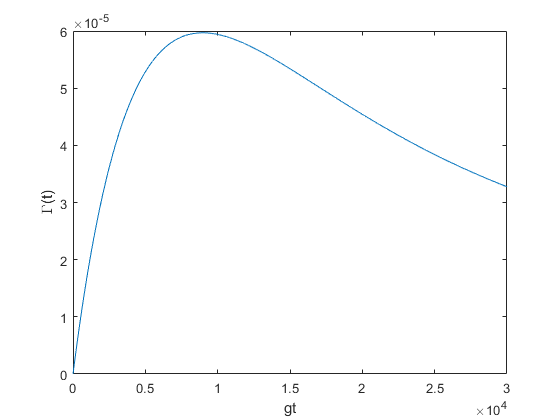
\includegraphics[width=0.35\textwidth]{plotted.png}}
                \caption{MATLAB program and the result of cocoa bean farm modification}
            \end{figure}
    \subsection{Other example}
        The is another mature example which is written by TokiNoBug. Here is the link of that article. \href{https://www.bilibili.com/read/cv8256187}{Calculated Nether Wart Farm}.

\begin{thebibliography}{99}
    \bibitem{ref1} \href{https://minecraft.fandom.com/wiki/Tick#Random_tick}{Wikipedia Minecraft}
\end{thebibliography}
\end{document}
